\documentclass[11pt]{article}
\usepackage[margin=1in]{geometry}
\usepackage[T1]{fontenc}
\usepackage[utf8]{inputenc}
\usepackage{lmodern,microtype,amsmath,amssymb,booktabs,graphicx,xcolor}
\usepackage[numbers,sort&compress]{natbib}
\usepackage[colorlinks=true,linkcolor=blue!50!black,citecolor=blue!50!black,urlcolor=blue!50!black]{hyperref}
\newtheorem{proposition}{Proposition}
\newtheorem{corollary}{Corollary}
% Generated by paper/make_numbers.py from result files; do not edit by hand.
\newcommand{\FbarDev}{0.020}
\newcommand{\GainPilot}{2.02}
\newcommand{\GfiveD}{0.23}
\newcommand{\GfiveDse}{0.09}
\newcommand{\GfiveF}{0.25}
\newcommand{\GfiveFse}{0.05}
\newcommand{\GfiveVmidF}{0.11}
\newcommand{\GfiveY}{\textminus{}0.57}
\newcommand{\GfiveYse}{0.28}
\newcommand{\HorizonT}{100}
\newcommand{\LR}{$5\times10^{-7}$}
\newcommand{\LRscoreA}{0.883}
\newcommand{\LRscoreB}{0.869}
\newcommand{\LRscoreC}{0.770}
\newcommand{\PilotValid}{12/12}
\newcommand{\PilotYvhighMax}{1.40}
\newcommand{\PilotYvhighMin}{0.53}
\newcommand{\PlanBV}{\textminus{}4.78}
\newcommand{\PowA}{0.08}
\newcommand{\PowB}{0.25}
\newcommand{\PowC}{0.43}
\newcommand{\PowPessA}{0.04}
\newcommand{\PowPessB}{0.09}
\newcommand{\PowPessC}{0.17}
\newcommand{\RhoMed}{\textminus{}0.41}
\newcommand{\RhoPess}{\textminus{}0.25}
\newcommand{\SigmaRraw}{0.220}
\newcommand{\SigmaS}{0.246}
\newcommand{\TVdeclared}{0.0177}
\newcommand{\TVpfail}{0.41}
\newcommand{\TVreplicate}{0.012}
\newcommand{\VRange}{0.172}
\newcommand{\VrankMin}{0.989}

\newcommand{\Fbar}{\overline{F}}
\newcommand{\fmax}{f_{\max}}
\newcommand{\qref}{q^{\mathrm{ref}}}

\title{Beyond Aggregate Verifier Quality:\\ Does Error-Mode Heterogeneity Predict RLVR Failure?\\[4pt]
\large A Pre-registered Matched-Rate Study}
\author{Alyssa L}
\date{Pre-registration: \url{https://osf.io/bs3wq/} (DOI 10.17605/OSF.IO/BS3WQ)\\ Code and data: \url{https://github.com/Alyssa-286/VERIFLOW}}

\begin{document}
\maketitle

\begin{abstract}
Reinforcement learning with verifiable rewards (RLVR) is usually analysed through a verifier's aggregate error rates.
Recent work shows that the \emph{pattern} of false positives, not only their rate, can decide whether training improves, plateaus or collapses.
We ask a narrower, quantitative question: among programmatic verifiers matched \emph{exactly} on the base-weighted aggregate false-acceptance rate $\Fbar$ and the true-positive rate $\tau$, does the dispersion $V$ of the per-error-mode false-acceptance probabilities predict the held-out accuracy reached by GRPO, beyond the worst-mode rate $\fmax$?
Replicator theory predicts that $V$ is the leading-order term at short horizon and that $\fmax$ dominates at long horizon.
We test this in one small, fully controlled setting: Qwen2.5-0.5B-Instruct on five-digit addition, with wrong answers partitioned into four outcome-defined modes and a verifier that accepts each mode at a designed rate.
A pilot confirmed that a high-$V$ verifier differentially amplifies its most-accepted mode within the pre-registered horizon of \HorizonT{} steps.
Because the pre-registered power analysis gave at most \PowC{} power, the confirmatory grid (48 configurations $\times$ 2 seeds) was registered as an \emph{estimation} study.
% Generated by paper/make_numbers.py; do not edit by hand.
All 96 of 96 registered runs completed and passed validation. Across the matched configurations, higher dispersion was associated with lower accuracy: $b_V=\ensuremath{-}6.01$ logit per unit $V$ (95\% CI \ensuremath{-}7.59 to \ensuremath{-}4.43), and the estimate is stable when the 11 duplicated verifier configurations that the registered grid contains are removed ($b_V=\ensuremath{-}5.63$, 95\% CI \ensuremath{-}8.30 to \ensuremath{-}2.95). Adding $V$ to $\fmax$ improved prediction of held-out configurations in the registered split (paired MSE difference \ensuremath{-}0.023, 95\% CI \ensuremath{-}0.047 to \ensuremath{-}0.002), but not on the 6 held-out verifiers that have no identical twin in training, and the CGF plug-in did not improve on $\{\fmax,V\}$. In exploratory analyses, the association is accompanied by a rise in the realised, on-policy false-acceptance rate (which the matched design-time rate does not capture) as the policy drifts toward the verifier's most-accepted error mode, and the lowest outcomes are single seeds that reward-hack one nearly always-accepted mode. With two seeds per configuration and one model and task, these are estimates for a narrow setting, not general claims.

All decisions, including a construct-validation stop, a census stability limitation and the downgrade to estimation, were logged before the data they govern; analyses added after the data are labelled as such.
\end{abstract}

\section{Introduction}
RLVR fine-tunes a language model on rewards from a programmatic checker: unit tests, an answer parser, a rule-based or model-based judge \citep{shao2024deepseekmath,yu2025dapo}.
Checkers make mistakes. A large literature models those mistakes as class-conditional noise characterised by a false-positive rate and a false-negative rate, or by Youden's index $J=\tau-\Fbar$ \citep{rad2026rate,cai2025reinforcement,mansouri2025noisecorrected}.
Under that block-symmetric view, all wrong answers are accepted with the same probability, and the drift of the incorrect mass depends on $J$ alone \citep{rad2026rate}.

Real checkers are not symmetric across wrong answers. They accept some \emph{kinds} of wrong answers far more often than others \citep{huang2025from,xin2026where,ray2026before}, and systematic false positives can produce plateaus or collapse that the overall error rate does not predict \citep{egashira2026delay}; a recent survey concludes that the structure of an error matters more than its rate \citep{gupta2026checking}.
What is missing is a \emph{quantitative} account: which summary of the per-mode acceptance profile predicts outcomes, at which horizon, once the aggregate rates are held fixed.

This paper isolates one such summary. For error modes $k$ with base-policy frequencies $\qref_k$ and verifier acceptance probabilities $f_k$, the aggregate rate is $\Fbar=\sum_k \qref_k f_k$ and the dispersion is $V=\sum_k \qref_k (f_k-\Fbar)^2$.
In the idealised replicator model, two verifiers with equal $\tau$ and $\Fbar$ differ in logit accuracy by $-\Delta V\,t^2/2$ to leading order (Section~\ref{sec:theory}), while at long horizon the most-accepted mode and $\fmax$ take over.
Whether this survives finite groups, shared parameters and Adam in a real transformer is an empirical question with no guaranteed sign.

\paragraph{Contributions.}
\begin{enumerate}
\item An exactly matched experimental design that varies $V$ and $\fmax$ while holding $\Fbar$ and $\tau$ fixed under the base-policy error distribution, with theory that reduces to the $J$-dynamics of \citet{rad2026rate} when $V=0$.
\item A pre-registered estimate, with confidence intervals, of the $V$--outcome association and of held-out-configuration prediction in one controlled RLVR setting (Qwen2.5-0.5B-Instruct, five-digit addition).
\item An empirical answer for this setting: at matched aggregate rates, dispersion is associated with lower accuracy ($b_V=\HoneBV$, 95\% CI \HoneLo{} to \HoneHi), predicts outcomes better than the aggregate or worst-mode rate, and coincides with drift toward the most-accepted error mode and occasional reward hacking (Sections~\ref{sec:results}--\ref{sec:robust}).
\item A transparent record of what did not work: a mechanism-based error taxonomy that reached its stop rule, a census stability criterion that proved noisy at the census size used, a confirmatory test downgraded to estimation for lack of power, and duplicated configurations in the registered grid that weaken the held-out test.
\end{enumerate}
We do \emph{not} claim that structure matters more than rate (that is established), nor anything about larger models, other tasks or natural verifiers.

\section{Related work}\label{sec:related}
\textbf{Noisy verifiers in RLVR.}
\citet{rad2026rate} derive replicator dynamics for GRPO under false positives and negatives and show a phase transition at $J=0$; their error model is symmetric across incorrect modes, so $V=0$ by construction.
\citet{cai2025reinforcement} and \citet{mansouri2025noisecorrected} study asymmetric but mode-independent noise and propose corrections.
\citet{plesner2026an} find RLVR on MBPP tolerant of resampled noise up to 20--30\%, and compare four \emph{correlation} structures (cell, row, column and whole-group flips) at equal rates; they do not vary acceptance by error mode.
\citet{moya2026verifier} analyse reward hacking under a fixed verifier and propose audit-based correction.

\textbf{Systematic false positives.}
\citet{egashira2026delay} show on arithmetic that systematic false positives cause outcomes ranging from delay to collapse that are not determined by the overall error rate. This is the closest work; it varies discrete false-positive patterns rather than a continuous dispersion statistic at exactly matched $\Fbar$ and $\tau$, and does not evaluate prediction on held-out configurations.
\citet{zhang2026when} contrast natural false positives in MBPP with hardened tests in a pre-registered design and find mechanism evidence consistent with selection of pre-existing error modes, the mechanism our model formalises.
Exploitable loopholes and reward hacking are studied by \citet{helff2026llms} and the CATCH testbed \citep{wang2026catch}; verifier audits that decompose errors by category include \citet{xin2026where}, \citet{ray2026before} and \citet{huang2025from}. Correlated errors within groups and across models \citep{xin2026are,kim2025correlated} motivate our per-sample pseudorandom verifier.

\textbf{Caveats from RLVR practice.} Qwen models can improve under spurious rewards \citep{shao2025spurious}, and fast reward saturation separates generalisation from memorisation \citep{rahman2026when}; both bear on our small, fast-saturating setting. We pin GRPO's loss and advantage scaling because of the biases documented by \citet{liu2025understanding}.

\section{Theory}\label{sec:theory}
Let the policy put probability $p_{\mathsf C}=A$ on correct answers and $p_k$ on incorrect class $k$, with $q_k=p_k/(1-A)$.
The verifier accepts a correct answer with probability $\tau$ and an answer of class $k$ with probability $f_k$.
Under the idealised assumptions (free categorical policy, natural-gradient replicator update with a common positive time change, exact expected rewards, no KL term, fixed classes), standard replicator results \citep{hofbauer1998evolutionary} give:

\begin{proposition}[closure and exact accuracy law]
$q_k(t)\propto q_k(0)e^{f_k t}$, independent of $\tau$ and $A(0)$, and
$\operatorname{logit}A(t)=\operatorname{logit}A(0)+\tau t-K_0(t)$ with $K_0(s)=\log\sum_k q_k(0)e^{s f_k}$.
\end{proposition}
\begin{proposition}[Fisher--Price]
$\frac{d}{dt}\sum_k q_k(t) f_k=\operatorname{Var}_{q(t)}(f)$; at $t=0$ the effective false-acceptance rate rises at rate exactly $V$.
\end{proposition}
\begin{corollary}[matched-rate contrast]
For verifiers with equal $\tau$ and equal $\Fbar$ under $\qref=q(0)$,
$\operatorname{logit}A_B(t)-\operatorname{logit}A_A(t)=-(V_B-V_A)\,t^2/2-(\kappa_{3,B}-\kappa_{3,A})\,t^3/6-\cdots$.
\end{corollary}
\begin{proposition}[long horizon]
As $t\to\infty$, $K_0(t)=\fmax t+\log q_{\arg\max f}(0)+o(1)$: if $\fmax>\tau$ accuracy collapses onto the most-accepted mode; otherwise $A\to1$ with a logit delay of $-\log q_{\arg\max f}(0)$.
\end{proposition}
Thus $V$ is the leading-order discriminator at short horizon and $\fmax$ at long horizon; the cumulant-generating-function (CGF) plug-in $Z(s)=\tau s-K(s)$ interpolates. Under vanilla softmax gradients the relevant statistic becomes a $q^2$-weighted covariance that can have the opposite sign (Proposition~7 of the Gate~1 report in the repository), so the theory does \emph{not} fix the sign of the $V$ effect for a transformer trained with Adam. These are standard results applied to verifier error, not new mathematics. All were checked numerically (21 tests; maximum error $\le10^{-10}$).

\textbf{Simulation (Gate 2).} In finite-group GRPO with stochastic verifiers, shared parameters and Adam (9 settings, 6 families, 3 horizons), adding $V$ to $\fmax$ reduced leave-one-configuration-out error in all 27 setting$\times$horizon cells (by 9--69\% of outcome variance), the coefficient of $V$ was negative in every family, and the CGF predictor gained value at longer horizons. Simulated classes are atomic actions, so this supports running the experiment; it is not evidence about language models.

\section{Experimental design}\label{sec:design}
\subsection{Task, error modes and construct validation}
The base model is Qwen2.5-0.5B-Instruct \citep{qwen2024qwen} at a pinned revision, asked to add two five-digit integers with an answer-only prompt.
Wrong answers are partitioned by how they differ from the true sum $S$: \textsf{LEN} (wrong digit count, including negatives), \textsf{ONE\_HI}/\textsf{ONE\_LO} (exactly one wrong digit in the high/low half), \textsf{MULTI} (two or more wrong digits), and \textsf{I} (unparseable).
This outcome-based partition (Amendment~1) replaced a pre-registered \emph{mechanism} taxonomy (dropped carry, transposition, \ldots) after that taxonomy reached its stop rule: 55--97\% of wrong answers matched no named mechanism across 24 censuses. The amendment and its timing are disclosed; its confirmatory census used operands never generated before.

The reference distribution $\qref$ was estimated from a census of 2{,}000 fresh prompts $\times$ 4 samples (base accuracy 0.349): \textsf{LEN} 0.162, \textsf{MULTI} 0.420, \textsf{ONE\_HI} 0.181, \textsf{ONE\_LO} 0.206, \textsf{I} 0.030.
A blinded 200-row audit of the classifier was labelled by an AI assistant from the written rules and reviewed by the author; it disagreed with the classifier on 1 row.

\textbf{Census stability limitation.} The pre-registered split-half total-variation criterion (TV $\le0.03$) was passed by the selected census (TV \TVdeclared), but a post hoc diagnosis showed the criterion is noisy at this census size: under random prompt halves the same census would exceed 0.03 with probability \TVpfail, because errors cluster strongly within prompts. The lock is supported instead by an independent-split replicate (TV \TVreplicate{} against the lock) and by bootstrap propagation: across the 48 registered configurations $\Fbar$ stays within $\pm$\FbarDev{} of 0.3 and the rank order of $V$ is preserved (Spearman $\ge$\VrankMin). A secondary 1.5B model failed the same criterion; no claim is made about it.

\subsection{Verifiers}
A verifier is a vector $(\tau,f_{\textsf{LEN}},f_{\textsf{MULTI}},f_{\textsf{ONE\_HI}},f_{\textsf{ONE\_LO}})$ with $f_{\textsf I}=0$; each decision is a Bernoulli draw from a SHA-256 pseudorandom function keyed on (verifier seed, run seed, step, prompt, sample), and every decision is logged.
\emph{Matched} configurations satisfy $\tau=0.9$ and $\Fbar=0.3$ exactly under $\qref$ (to $10^{-12}$); $V$ and $\fmax$ vary over a grid of $V$ fractions $\{0,.25,.5,.75,1\}$ of the feasible range $\times$ $\fmax\in\{\text{free},0.6,0.95\}$, with the mode carrying $\fmax$ randomised. \emph{Auxiliary} configurations use $\Fbar\in\{0.15,0.45\}$.

\subsection{Training and outcome}
GRPO with the DAPO loss \citep{yu2025dapo}, no KL term, group reward scaling, $G=8$ samples for each of 32 prompts per step, neutral sampling, full fine-tuning with AdamW at a constant learning rate, implemented in TRL 1.17.1. The learning rate (\LR) and horizon ($T=\HorizonT$ steps) were set by pre-declared rules on a learning-rate pilot.
The primary outcome of a run is $Y=\operatorname{logit}$ of the mean greedy accuracy on 1{,}000 held-out prompts over the evaluations in $[T/2,T]$ (every 10 steps, six points). The configuration outcome $\bar Y$ is the mean over two seeds.

\subsection{Pilot, power and the registered claim}
A heterogeneity pilot (4 configurations $\times$ 3 seeds, \PilotValid{} runs valid) was evaluated with a pre-declared engagement rule (Gate~5). The high-$V$ verifier amplified its most-accepted mode beyond the homogeneous control (log-growth difference \GfiveD, SE \GfiveDse) and raised the realised acceptance of wrong rollouts (\GfiveF, SE \GfiveFse), so the manipulation reaches the policy within $T$ (Figure~\ref{fig:pilot}).
The pre-registered power simulation used the pilot's seed SD (\SigmaS{} logit) and an effect size transferred from the simulation (median share $\rho=\RhoMed$ of the homogeneous logit gain). Power for the $V$ coefficient at the Holm-adjusted level $\alpha=0.05/3$ was \PowA, \PowB{} and \PowC{} for 12, 24 and 36 matched configurations (pessimistic effect: \PowPessA, \PowPessB, \PowPessC).
Following the rule fixed in advance, the study uses the largest design (36 matched + 12 auxiliary configurations, 96 runs) and reports \emph{estimates with confidence intervals}; $p$-values are reported but not interpreted as confirmatory.

\begin{figure}[t]
\centering
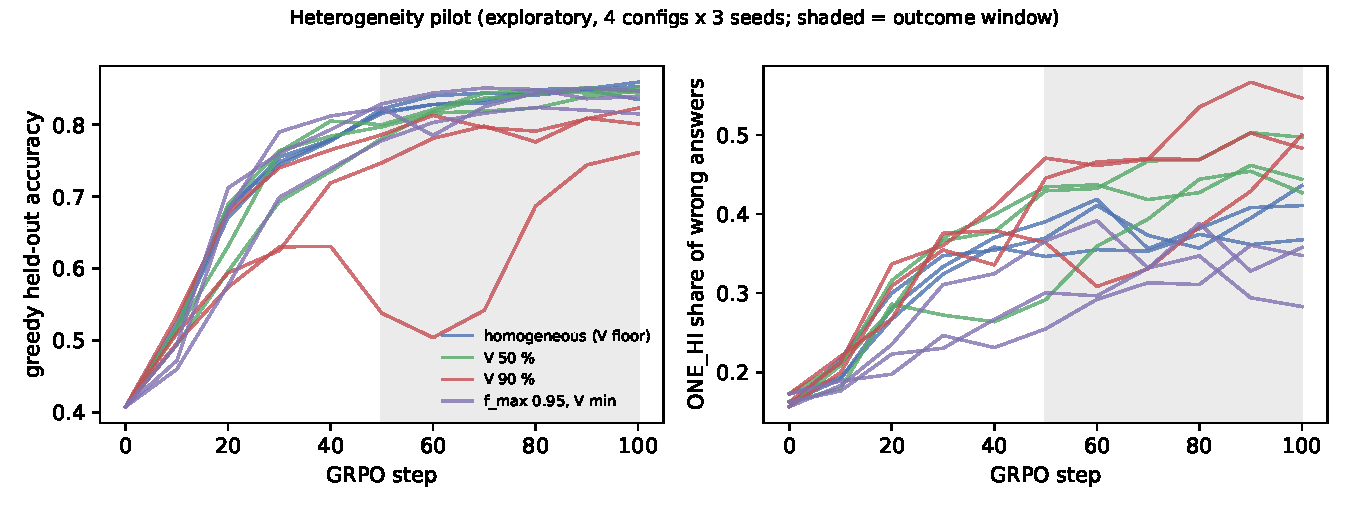
\includegraphics[width=\linewidth]{../figures/out/fig_pilot_het.pdf}
\caption{Heterogeneity pilot (exploratory; 4 configurations $\times$ 3 seeds). Left: greedy held-out accuracy. Right: share of \textsf{ONE\_HI}, the high-$V$ verifier's most-accepted mode, among wrong answers. Shaded: outcome window. One high-$V$ seed collapses inside the window before recovering.}
\label{fig:pilot}
\end{figure}

\subsection{Pre-registered analysis}
H1: in the matched arm, $\bar Y_r=b_0+b_V V_r+b_f f_{\max,r}+\varepsilon_r$ with HC3 standard errors.
H2: on 13 held-out configurations, compare the squared prediction error of $\{\fmax,V\}$ against $\{\fmax\}$, both fitted on the 23 training configurations, with a 10{,}000-resample configuration-level bootstrap.
H3: the same comparison for the CGF plug-in $Z(s)$ ($s$ chosen by cross-validation) against $\{\fmax,V\}$.
Holm adjustment over H1--H3; ICC between configuration and seed; exploratory comparison of every registered predictor across both arms.
The registration (\url{https://osf.io/bs3wq/}) was recorded before the first confirmatory run started.

\subsection{Deviations and post-registration analyses}
No registered hypothesis, outcome, unit, test, threshold, seed, configuration or exclusion rule was changed, and no run was excluded. Four things were added after the data and are labelled wherever they appear: (i) the coefficient $b_f$ and the realised verifier rates, which the registration lists but the pre-written analysis driver did not print; (ii) the registered all-arm secondary model, in which $J$ and $J_{\text{worst}}$ (the registered ``conditional advantage'') are exact aliases of the aggregate rate and $\fmax$ because $\tau$ is constant; (iii) the discovery that the registered grid contains duplicated verifiers, with deduplicated sensitivity analyses; and (iv) post hoc comparisons of aggregate rates with dispersion, robustness checks and a description of unusual runs. The scripts for (i)--(iv) were written after the registered analysis had been run (\texttt{experiments/analyse\_grid\_supplement.py}, decision D33 in the repository).

% Hand-written text; every number is a macro from generated/numbers.tex (paper/make_numbers.py).
\section{Confirmatory results}\label{sec:results}

\subsection{Execution and validity}
All \GridValid{} of \GridRuns{} registered runs (48 configurations $\times$ 2 seeds, Slurm array 4036, one commit, two runs at a time on two L40 GPUs) completed and passed every validation check: run status and final step, learning rate, seed, horizon and evaluation cadence, the SHA-256 of each verifier configuration against its registered file, the $\qref$ lock hash, a clean source tree, the evaluation schedule, and a complete verifier decision log. The digest of the configuration directory equals the value committed in the registration. No run was rerun, excluded or replaced, and no run diverged (\Divergences{} runs met the registered divergence definition). Training used \GPUhours{} GPU-hours at a median of \StepSecMed{}~s per step.

\textbf{Realised verifier rates.} The verifier logs record every decision. The realised acceptance rate of correct rollouts was between \TaurealMin{} and \TaurealMax{} in every run, matching $\tau=0.9$. Over all training steps, the realised false-acceptance rate on wrong rollouts in the matched arm averaged \FrealAllMatched{}, against the design value 0.3 under $\qref$; in the outcome window it ranged from \FrealMatchedMin{} to \FrealMatchedMax{} across runs (mean \FrealMatchedMean). This spread is expected: $\Fbar$ is matched under the \emph{base} error distribution, and the policy's error distribution moves during training (Proposition~2). The window rate is rank-correlated with $V$ (Spearman \SpearFrealV), so it is a post-treatment quantity, not a covariate.

\textbf{Disclosure: duplicated verifier configurations.} After the registered analysis was run, we found that the registered grid contains exact duplicates. The generator drew three candidates per grid cell, and in several cells the constraints fix the acceptance vector up to the choice of mode, so some candidates coincide; for example, every $V$-fraction-0 cell yields the homogeneous verifier. The 36 matched configurations contain \NuniqueMatched{} distinct verifiers (\NdupGroups{} groups of duplicates), and the 48 configurations contain \NuniqueAll. Because a run is a deterministic function of the verifier, the seed and the evaluation cadence, duplicated configurations produced bit-identical outcomes. Two consequences matter: the registered H1 treats 36 rows as independent when 25 are distinct, which understates its standard error; and \NheldTwin{} of the \NheldOut{} held-out configurations have an identical twin among the training configurations, so part of the registered held-out comparison is not out-of-configuration. The registered analysis is reported unchanged below. Each primary quantity is then re-estimated on distinct verifiers only, as a sensitivity analysis labelled exploratory (Section~\ref{sec:robust}).

\subsection{Registered estimates}

\begin{table}[t]
\centering
\caption{Registered primary estimates (matched arm, configuration = unit). The registration declared these estimates with confidence intervals as the primary results; $p$-values are reported but not interpreted as confirmatory tests (power was below 0.5). MSE differences are paired, negative values favour the first predictor set.}
\label{tab:primary}
\small
\begin{tabular}{@{}llll@{}}
\toprule
Quantity & Estimate & 95\% CI & $p$ (Holm) \\
\midrule
H1: $b_V$ (HC3, $n=36$, df 33) & \HoneBV & [\HoneLo, \HoneHi] & \HoneP{} (\HolmHone) \\
H1: $b_f$ (same fit) & \HoneBF & [\HoneBFLo, \HoneBFHi] & -- \\
H2: MSE$\{\fmax,V\}$ $-$ MSE$\{\fmax\}$, 13 held out & \HtwoDiff & [\HtwoLo, \HtwoHi] & \HtwoP{} (\HolmHtwo) \\
H3: MSE$\{Z(s)\}$ $-$ MSE$\{\fmax,V\}$, $s=\HthreeS$ & \HthreeDiff & [\HthreeLo, \HthreeHi] & \HthreeP{} (\HolmHthree) \\
\midrule
\multicolumn{4}{@{}l}{\emph{Sensitivity, distinct verifiers only (exploratory)}}\\
H1: $b_V$ ($n=\NuniqueMatched$, df 22) & \UniqBV & [\UniqBVLo, \UniqBVHi] & -- \\
H1: $b_f$ & \UniqBF & [\UniqBFLo, \UniqBFHi] & -- \\
Leave-one-verifier-out: $\{\fmax,V\}-\{\fmax\}$ & \UniqDiff & [\UniqDiffLo, \UniqDiffHi] & \UniqDiffP \\
Leave-one-verifier-out: $\{Z(s)\}-\{\fmax,V\}$ & \UniqZDiff & [\UniqZDiffLo, \UniqZDiffHi] & -- \\
Held out without twins ($n=\PureN$): H2 difference & \PureDiff & [\PureLo, \PureHi] & -- \\
\bottomrule
\end{tabular}
\end{table}

\textbf{H1 (dispersion at matched rates).} Across the 36 matched configurations, $\bar Y$ decreased with $V$ at fixed $\fmax$: $b_V=\HoneBV$ logit per unit of $V$ (HC3 95\% CI \HoneLo{} to \HoneHi; Table~\ref{tab:primary}, Figure~\ref{fig:h1}). Over the realised range of $V$ (0 to about 0.17), this corresponds to roughly one logit unit of window accuracy. The fit explains $R^2=\HoneRsq$ of the between-configuration variance, and the rank correlation of $\bar Y$ with $V$ is \SpearmanYV. With $V$ in the model, the worst-mode rate has a small positive coefficient ($b_f=\HoneBF$, CI \HoneBFLo{} to \HoneBFHi), which does not survive deduplication. The point estimate is close to the planning value used for the power analysis ($b_V=\PlanBV$), but the interval is much narrower than that analysis anticipated. The power simulation set the between-configuration SD to the pilot's seed SD (\SigmaS) as a conservative floor and added seed noise on top. In the grid, seed noise is heavy-tailed: most seed pairs differ by little (median gap \SeedGapMed{} logit), while a few high-$V$ pairs differ by more than one logit (Section~\ref{sec:results}, mechanism), so the one-way ICC is only \ICCmatched{} even though $V$ and $\fmax$ explain most of the between-configuration variance. The precision of $b_V$ is a property of this grid and should not be read as evidence that the planning noise model was wrong in general.

\textbf{H2 (held-out prediction beyond $\fmax$).} Fitted on the 23 training configurations, $\{\fmax,V\}$ predicted the 13 held-out configurations with MSE \HtwoMSEfv, against \HtwoMSEf{} for $\fmax$ alone (difference \HtwoDiff, CI \HtwoLo{} to \HtwoHi; Holm-adjusted $p$ \HolmHtwo; Figure~\ref{fig:heldout}). Leave-one-configuration-out MSE on all matched configurations agrees (\LocoFV{} vs \LocoF).

\textbf{H3 (CGF plug-in).} The CGF predictor, with $s$ chosen by cross-validation on the training configurations ($s=\HthreeS$, the smallest grid value, where $Z(s)$ is close to its second-order expansion in $V$), predicted as well as $\{\fmax,V\}$ but not better (difference \HthreeDiff, CI \HthreeLo{} to \HthreeHi).

\begin{figure}[t]
\centering
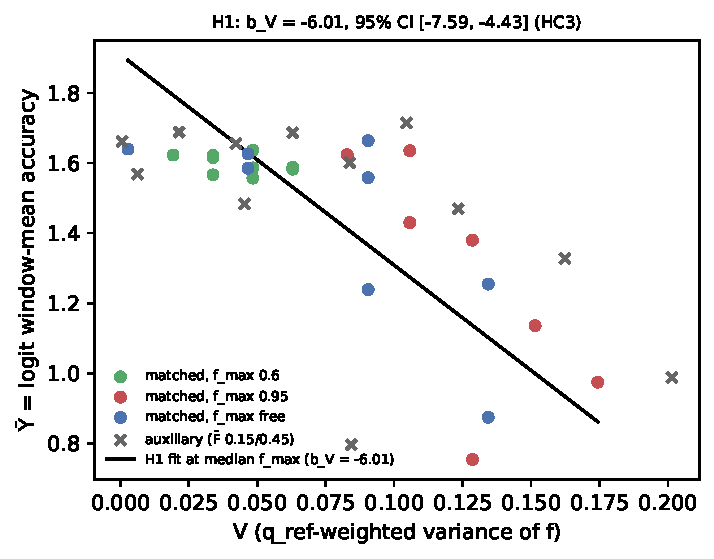
\includegraphics[width=0.62\linewidth]{../figures/out/fig_grid_h1.pdf}
\caption{Configuration-mean outcome against $V$. Matched configurations are coloured by $\fmax$ level; auxiliary configurations ($\Fbar=0.15$ or $0.45$) are crosses. Line: registered H1 fit at the median $\fmax$. Duplicated configurations plot on top of each other.}
\label{fig:h1}
\end{figure}

\subsection{Secondary outcomes and mechanism}
Mean final accuracy was \AccTmatched{} in the matched and \AccTaux{} in the auxiliary arm, from 0.408 at step 0. The registered hacking indicator (final accuracy at least 0.029 below the run's peak) fired in \NhackRuns{} of 96 runs. Figure~\ref{fig:modes} shows the mechanism the theory describes: under low-$V$ and homogeneous verifiers, the share of the most-accepted mode among errors falls during training, while under high-$V$ verifiers it rises, reaching about 0.4 of all errors in the outcome window.

The lowest outcomes come from single seeds. \NlowHighV{} matched runs from high-$V$ configurations (\NlowDistinct{} distinct trajectories once duplicates are merged, plus \NlowAux{} auxiliary run) have $Y<0.3$; no low-$V$ run does. In each, the most-accepted mode is \textsf{LEN}, accepted with probability about 0.95. Accuracy first rises with the control, peaks near step 40, then falls to \LowAccT{} while \textsf{LEN} grows to \LowLenT{} of the errors (Figure~\ref{fig:supp}b): the policy learns to produce wrong-length answers that the verifier nearly always accepts. The other seed of the same configuration did not do this within 100 steps. Within-configuration seed gaps are small in general (median \SeedGapMed{} logit) but grow with $V$ (Spearman \SeedGapRho{} in the matched arm). Higher dispersion therefore adds both a lower mean and a larger chance of a hacking episode within the horizon. Two seeds per configuration cannot estimate that chance.

\begin{figure}[t]
\centering
\begin{minipage}{0.49\linewidth}\centering
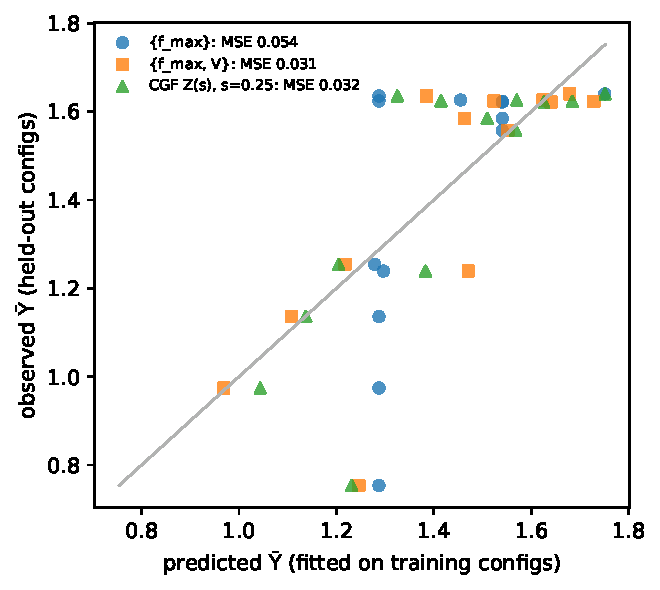
\includegraphics[width=\linewidth]{../figures/out/fig_grid_heldout.pdf}
\caption{Registered held-out comparison (H2/H3): predictions of the 13 held-out configurations from models fitted on the 23 training configurations.}
\label{fig:heldout}
\end{minipage}\hfill
\begin{minipage}{0.49\linewidth}\centering
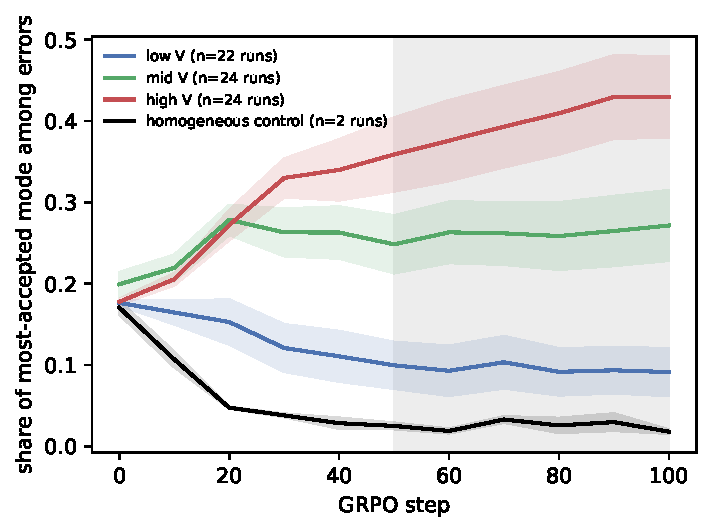
\includegraphics[width=\linewidth]{../figures/out/fig_grid_modes.pdf}
\caption{Share of each configuration's most-accepted mode among wrong answers (sampled census on 1{,}000 prompts), by $V$ tertile, matched arm, mean $\pm$ SE over runs. Shaded: outcome window.}
\label{fig:modes}
\end{minipage}
\end{figure}

\section{Aggregate verifier quality versus heterogeneity}\label{sec:aggregate}
The matched arm holds the aggregate rates fixed, so there H1 already measures dispersion beyond aggregate quality. The registered secondary analysis lets the aggregate rate vary across both arms ($n=\SecN$ configurations, $\Fbar\in\{0.15,0.3,0.45\}$, $\tau=0.9$ throughout). All comparisons in this section are labelled exploratory: they are either registered secondary analyses without a pre-specified test or, where noted, post hoc.

\textbf{Single predictors.} Leave-one-configuration-out MSE relative to the variance of $\bar Y$ (lower is better; 1.0 is no better than the mean): $V$ \RelV, $V_{q^2}$ \RelVqtwo, CGF \RelCGF, $\fmax$ \RelFmax, $\kappa_3$ \RelKappa, $\max_k q_kf_k$ \RelMaxqf, trigger frequency \RelTrig, intercept only \RelNull{} (Figure~\ref{fig:pred}). The design aggregate false-acceptance rate alone reaches \RelAggF.

\textbf{Nested models (post hoc).} Adding $\fmax$ to the aggregate rate gives \RelAggFM; adding $V$ instead gives \RelAggFV; with all three, \RelAggFMV, and the coefficient of $V$ is \AggFMVcoefV{} (CI \AggFMVcoefVLo{} to \AggFMVcoefVHi), while that of the aggregate rate is \AggFMVcoefF{} (CI \AggFMVcoefFLo{} to \AggFMVcoefFHi). On distinct verifiers only, the relative MSE is \UniqRelFM{} without and \UniqRelFMV{} with $V$, and the $V$ coefficient is \UniqAggV{} (CI \UniqAggVLo{} to \UniqAggVHi). Over this range of aggregate rates, dispersion carries more information about the outcome than the aggregate rate does.

\textbf{Registered joint model.} The registered secondary model with all estimable predictors (aggregate rate, $\fmax$, trigger frequency, $V$, $\kappa_3$, $V_{q^2}$, $\max_k q_kf_k$; $J$ and $J_{\text{worst}}$ are exact aliases of the aggregate rate and $\fmax$ when $\tau$ is constant) predicts with relative MSE \SecRel, but its predictors are highly collinear (variance inflation factor of $V$: \SecVifV), so no single coefficient is identified: $b_V=\SecV$ (CI \SecVLo{} to \SecVHi). We do not interpret its coefficients.

\textbf{Realised rate (post hoc).} The realised window false-acceptance rate alone predicts better than any design statistic (relative MSE \RelAggR; with $\fmax$ and $V$, \RelAggRMV). In H1 with the realised rate added, $b_V$ shrinks from \HoneBV{} to \MedBV{} (CI \MedBVLo{} to \MedBVHi). Because the realised rate is itself moved by $V$ (Figure~\ref{fig:supp}a), this is a mediator, not a confounder: the result is consistent with dispersion acting largely by raising the on-policy false-acceptance rate as the policy shifts toward accepted modes. It does not show that the realised rate is a usable design-time predictor, because it is only known after training.

\begin{figure}[t]
\centering
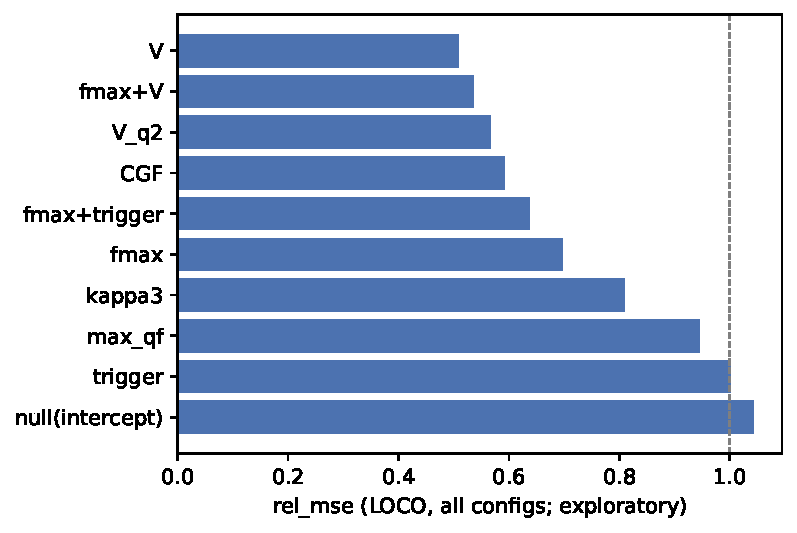
\includegraphics[width=0.5\linewidth]{../figures/out/fig_grid_predictors.pdf}
\caption{Leave-one-configuration-out MSE relative to $\operatorname{Var}(\bar Y)$ for every registered predictor set, all 48 configurations (exploratory).}
\label{fig:pred}
\end{figure}

\begin{figure}[t]
\centering
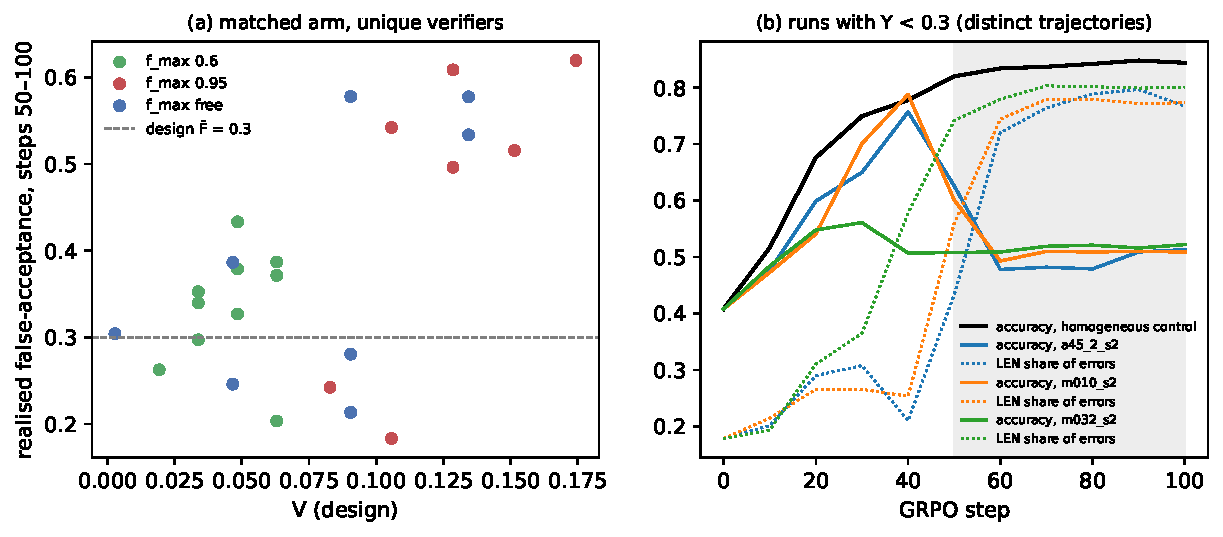
\includegraphics[width=\linewidth]{../figures/out/fig_grid_supp.pdf}
\caption{(a) Realised false-acceptance rate on wrong rollouts in the outcome window against design $V$ (matched arm, distinct verifiers). (b) Runs with $Y<0.3$: accuracy (solid) and \textsf{LEN} share of errors (dotted) against the homogeneous control. Exploratory.}
\label{fig:supp}
\end{figure}

\section{Robustness and sensitivity}\label{sec:robust}
The three registered robustness re-fits of H1 (labelled exploratory in the registration) agree with the primary estimate: without the homogeneous control $b_V=\RobNoHomBV$ (CI \RobNoHomLo{} to \RobNoHomHi); on final rather than window accuracy $b_V=\RobFinalBV$ (CI \RobFinalLo{} to \RobFinalHi); and with only configurations that have two valid seeds the fit is identical, because no run was lost. Post hoc checks:
\begin{itemize}
\item \emph{Distinct verifiers} (the duplicate disclosure above): $b_V=\UniqBV$ (CI \UniqBVLo{} to \UniqBVHi, df 22). Leave-one-verifier-out over the \NuniqueMatched{} distinct matched verifiers still favours $\{\fmax,V\}$ over $\{\fmax\}$ (MSE \UniqLooFV{} vs \UniqLooF; paired difference \UniqDiff, CI \UniqDiffLo{} to \UniqDiffHi), and the CGF is again equal to $\{\fmax,V\}$ (\UniqLooZ). On the \PureN{} registered held-out verifiers that have no twin in training, the H2 difference is \PureDiff{} (CI \PureLo{} to \PureHi): with six configurations this comparison is uninformative, and it does not reproduce the registered H2 advantage.
\item \emph{Influence}: dropping any one configuration moves $b_V$ between \LooBVmin{} and \LooBVmax.
\item \emph{Run-level model} with configuration-clustered standard errors: $b_V=\ClustBV$ (CI \ClustLo{} to \ClustHi).
\item \emph{Rank-based}: partial Spearman correlation of $\bar Y$ and $V$ given $\fmax$, \PartialSpear.
\item \emph{Hacking episodes}: removing the runs with $Y<0.3$ (a sensitivity check only; the registered estimate keeps every run) gives $b_V=\NoLowBV$ (CI \NoLowBVLo{} to \NoLowBVHi), so the association is not carried by the few hacking runs alone.
\end{itemize}

% Hand-written text; numbers are macros from generated/numbers.tex.
\section{Discussion}\label{sec:discussion}
\textbf{Answer to the question.} In this setting, error-mode heterogeneity predicts RLVR outcome beyond aggregate verifier quality. Verifiers with exactly the same base-weighted false-acceptance rate and the same true-positive rate led to different accuracy, ordered by the dispersion $V$ of their per-mode acceptance probabilities, with a precise negative estimate that survives deduplication, influence checks, a run-level model and a rank-based check. Across three aggregate rates, $V$ predicted left-out configurations better than the aggregate rate or the worst-mode rate (exploratory). The pre-registered competitors did not beat it: $\fmax$ added little once $V$ was known, and the CGF plug-in, which theory suggests should gain at longer horizons, chose the smallest horizon on its grid and matched $V$ without improving on it. At $T=\HorizonT$ steps this is the short-horizon regime in which the replicator expansion makes $V$ the leading term (Section~\ref{sec:theory}). The sign of the effect was not guaranteed by theory, since the vanilla-gradient statistic can reverse it; here it is the replicator sign.

\textbf{What the evidence does not show.} First, the registered held-out test (H2) favoured $V$, but \NheldTwin{} of its \NheldOut{} held-out configurations duplicate training configurations; on the \PureN{} that do not, the comparison is uninformative. The leave-one-verifier-out comparison over distinct verifiers supports H2's direction, but it was not the registered test. Second, every $p$-value was declared non-confirmatory in advance; we report the H1 interval as an estimate and do not convert it into a confirmatory rejection after the fact. Third, the mechanism analysis is exploratory. The rise of the most-accepted mode and of the realised false-acceptance rate with $V$, and the hacking episodes on a nearly always-accepted mode, are consistent with the selection mechanism in the theory, but they were not registered tests.

\textbf{Practical reading.} A verifier's aggregate false-positive rate, measured on the base policy, is not a sufficient description of its risk. Two checks with the same measured rate can differ in how much they reward a single kind of wrong answer, and RL finds and amplifies that kind. Reporting the per-mode acceptance profile, or at least its dispersion and maximum, is cheap when error modes can be classified, and it predicted outcomes here where the aggregate did not. Monitoring the realised, on-policy false-acceptance rate during training is a direct way to see the drift.

\section{Limitations}\label{sec:limits}
\begin{itemize}
\item \textbf{Scope.} One model (Qwen2.5-0.5B-Instruct), one task (five-digit addition), four outcome-defined error modes, synthetic Bernoulli verifiers, $T=\HorizonT$ GRPO steps, one learning rate. Nothing here licenses claims about larger models, other tasks, natural verifiers or long training. In particular, the long-horizon regime, where theory predicts that $\fmax$ takes over, was not reached.
\item \textbf{Two seeds per configuration}, as registered. Seed-to-seed spread grows with $V$, and the hacking episodes occurred in one seed of a pair; their frequency cannot be estimated from two seeds.
\item \textbf{Power and claim type.} The registered power for H1 at the strictest Holm threshold was \PowC{} (pessimistic \PowPessC). The study was therefore registered as estimation with confidence intervals, and it is reported that way, although the observed interval turned out to be narrow.
\item \textbf{Duplicated configurations.} The registered grid has \NuniqueMatched{} distinct matched verifiers, not 36. Registered standard errors and the registered held-out test are affected; the deduplicated analyses are post hoc.
\item \textbf{Census stability.} The reference distribution passed the registered split-half criterion, but that criterion would fail for the same census under \TVpfail{} of random prompt splits. The lock is supported by an independent replicate and by bootstrap propagation ($\Fbar$ within $\pm$\FbarDev{} of 0.3), so the matching of aggregate rates holds to about $\pm0.02$, not exactly, at the true base distribution.
\item \textbf{1.5B model.} A secondary Qwen2.5-1.5B arm failed the same stability criterion (TV 0.039 and 0.050 against 0.03). A post hoc diagnosis attributes this to sampling variability under strong within-prompt clustering, but the declared failure stands, no 1.5B reference distribution exists, and no 1.5B result is reported.
\item \textbf{Pilot.} The heterogeneity pilot used 4 configurations $\times$ 3 seeds and is descriptive. Its effect size was not used for planning; the planning effect came from simulation.
\item \textbf{Taxonomy and audit.} The registered mechanism taxonomy reached its stop rule and was replaced, before any training data, by an outcome-defined partition (Amendment~1). The 200-row construct audit was labelled by an AI assistant from written rules and reviewed by the author.
\item \textbf{Literature coverage.} Forward-citation search was rate-limited, so recent work citing the closest papers may be missing from the related-work review.
\end{itemize}

\section{Conclusion}\label{sec:conclusion}
In a pre-registered, exactly rate-matched study of GRPO on Qwen2.5-0.5B-Instruct and five-digit addition, verifiers that spread the same false-acceptance budget unevenly across error modes led to lower accuracy, and the dispersion statistic $V$ predicted outcomes better than the aggregate rate or the worst-mode rate. The study was registered as an estimation study and is reported as one; the held-out test is weakened by duplicated configurations in the registered grid, and the evidence is confined to one small model, one task and a short horizon. The code, the registration, every decision and all run records are public so that the estimate can be checked and extended.

\paragraph{Data and code availability.} The pre-registration is DOI 10.17605/OSF.IO/BS3WQ (\url{https://osf.io/bs3wq/}). Code, configurations, run records, analysis outputs and the decision log are at \url{https://github.com/Alyssa-286/VERIFLOW}. Model checkpoints are not archived (about 1.1~TB); every run can be regenerated from its configuration and seed.

\paragraph{Use of AI assistance.} Code, analyses and text were developed with an AI coding assistant (Claude) under the author's direction; the construct audit labels are disclosed above. All results come from the logged runs and scripts in the repository.


\bibliographystyle{plainnat}
\bibliography{references}
\end{document}
